\chapter{Data and Methodology}
\label{chap:met}

\section{Data}

	I obtain the dataset from \cite{tobek2020does}. The dataset comprises of liquid publicly traded shares from developed countries of Europe, Japan and Asia-Pacific (Australia, New Zealand, Hong Kong, and Singapore). The data is monthly and spans from 1990 to 2018. I use the liquid universe, which contains 8,350 companies,  totaling 1,607,117 observations. 
	
	This thesis uses 30 anomalies that were identified as strongest predictors of equity returns in the \cite{tobek2020does} paper. The authors compute 153  anomalies, firm-level characteristics that have been put forward by leading financial and accounting journals as predictors of equity returns. The authors then use the 153 anomalies in a single model, which allows individual effects to crowd each other out, and results in ordering of the predictors from the strongest to the weakest. This thesis takes 30 predictors identified as strongest on liquid global universe of stocks (Figure 8 in \cite{tobek2020does}).
	
	Table [TODO add summary table] shows the 30 anomalies studied. 
	
	I preprocess all predictors in the following manner (in line with \cite{gu2020empirical}). First, I winsorize bottom and top 1\% of each variable to mitigate the impact of observations with implausibly large or small values. Second, I center each variable so that its mean is 0 and subsequently normalize so that the resulting values lie between -1 and 1. This is done because neural networks work better with data on the same scale. Finally, I impute missing values by mean (that is, 0), as all values entering a neural network must be numerical and the value 0 can be interpreted as "no information". I perform all these operations on data grouped by year, that is, first split the data into groups by year, then apply the transformations and finally combine back into single dataset. The main motivation for this is to prevent information from getting from test sets to training and validation sets.    	
	
	Table \ref{tab:descr} shows descriptive statistics of the anomalies data after these transformations.
		
	Figure \ref{fig:corrplot}, shows plot of the correlation matrix of the anomalies.

	The task is to predict the return of given stock in month $t+1$ given that stock's anomalies as of the time $t$. (Two technical notes: first, the dataset is organized so that this shift is taken care of, i.e., the features corresponding to the given target have the same index. Second, the anomalies as of the time $t-1$ can be (and often are) calculated from raw data based on several preceding time periods, e.g., $t$, $t-1$, $t-2$ and therefore the time index  represents the entire information set rather than financial or accounting information being \textit{published} at that time index. For example, a single observation at a given time index $t$ consists of the target (stock's return in $t+1$), and anomalies calculated as of $t$, such as average return in the last six months ($t$, $t-1$, $t-2$, $t-3$, $t-4$, $t-5$))
	
	Figure \ref{fig:hist_returns} shows histogram of the targets (monthly returns). 
	
	
	

	%\begin{tabular}{lrrrrrrrr}
\toprule
{} &      count &  mean &     std &     min &     25\% &     50\% &     75\% &    max \\
\midrule
Lagged Momentum                            &  1607088.0 &   0.0 &  0.0316 & -0.1518 & -0.0053 & -0.0009 &  0.0029 &  1.000 \\
Seasonality                                &  1607088.0 &  -0.0 &  0.0282 & -0.2622 & -0.0034 & -0.0002 &  0.0021 &  1.000 \\
Short-Term Reversal                        &  1607088.0 &  -0.0 &  0.2430 & -0.9831 & -0.1276 & -0.0178 &  0.1027 &  1.000 \\
Momentum-Reversal                          &  1607088.0 &   0.0 &  0.0200 & -0.0802 & -0.0054 & -0.0008 &  0.0029 &  1.000 \\
52-Week High                               &  1607088.0 &  -0.0 &  0.3316 & -1.0000 & -0.1828 &  0.0764 &  0.2445 &  0.678 \\
RD / Market Equity                         &  1607088.0 &  -0.0 &  0.0169 & -0.0311 & -0.0001 &  0.0000 &  0.0000 &  1.000 \\
Liquidity Shocks                           &  1607088.0 &  -0.0 &  0.0055 & -0.0016 & -0.0001 & -0.0001 & -0.0000 &  1.000 \\
Earnings Predictability                    &  1607088.0 &   0.0 &  0.0158 & -0.0081 & -0.0006 &  0.0000 &  0.0000 &  1.000 \\
Seasonality 6-10 A                         &  1607088.0 &  -0.0 &  0.0220 & -0.1208 & -0.0055 &  0.0000 &  0.0029 &  1.000 \\
Change in Common Equity                    &  1607088.0 &  -0.0 &  0.0153 & -0.0199 & -0.0013 & -0.0003 & -0.0001 &  1.000 \\
Seasonality 6-10 N                         &  1607088.0 &   0.0 &  0.0220 & -0.1307 & -0.0050 &  0.0000 &  0.0020 &  1.000 \\
Seasonality 2-5 N                          &  1607088.0 &   0.0 &  0.0219 & -0.1313 & -0.0061 & -0.0005 &  0.0035 &  1.000 \\
Seasonality 2-5 A                          &  1607088.0 &  -0.0 &  0.0180 & -0.1002 & -0.0042 & -0.0000 &  0.0027 &  1.000 \\
Leverage Component of Book/Price           &  1607088.0 &   0.0 &  0.0089 & -0.0057 & -0.0002 & -0.0001 & -0.0000 &  1.000 \\
Amihud's Measure (Illiquidity)             &  1607088.0 &   0.0 &  0.0221 & -0.0113 & -0.0005 & -0.0002 & -0.0001 &  1.000 \\
Profit Margin                              &  1607088.0 &   0.0 &  0.0652 & -1.0000 & -0.0000 &  0.0011 &  0.0097 &  1.000 \\
Volume Trend                               &  1607088.0 &   0.0 &  0.2040 & -0.8532 & -0.0873 &  0.0000 &  0.0979 &  1.000 \\
Coefficient of Variation of Share Turnover &  1607088.0 &  -0.0 &  0.1144 & -0.1469 & -0.0625 & -0.0279 &  0.0170 &  1.000 \\
Earnings Forecast-to-Price                 &  1607088.0 &   0.0 &  0.0137 & -0.1066 & -0.0006 &  0.0000 &  0.0000 &  1.000 \\
Duration of Equity                         &  1607088.0 &   0.0 &  0.0624 & -1.0000 & -0.0006 &  0.0000 &  0.0068 &  1.000 \\
Seasonality 11-15 N                        &  1607088.0 &   0.0 &  0.0213 & -0.1246 & -0.0032 &  0.0000 &  0.0005 &  1.000 \\
Operating Profits to Assets                &  1607088.0 &   0.0 &  0.0562 & -0.3581 & -0.0122 &  0.0000 &  0.0011 &  1.000 \\
Max                                        &  1607088.0 &   0.0 &  0.1913 & -0.2571 & -0.1111 & -0.0544 &  0.0416 &  1.000 \\
Whited-Wu Index                            &  1607088.0 &   0.0 &  0.1681 & -0.7012 & -0.0528 &  0.0000 &  0.0489 &  1.000 \\
Net Operating Assets                       &  1607088.0 &  -0.0 &  0.0171 & -0.0869 & -0.0007 & -0.0001 &  0.0000 &  1.000 \\
Accruals                                   &  1607088.0 &   0.0 &  0.0484 & -0.3996 & -0.0043 &  0.0000 &  0.0033 &  1.000 \\
Idiosyncratic Risk                         &  1607088.0 &  -0.0 &  0.1999 & -0.2929 & -0.1204 & -0.0539 &  0.0528 &  1.000 \\
Coskewness                                 &  1607088.0 &  -0.0 &  0.1996 & -1.0000 & -0.1014 &  0.0000 &  0.1074 &  1.000 \\
Liquidity Beta 5                           &  1607088.0 &  -0.0 &  0.0724 & -0.3288 & -0.0298 &  0.0000 &  0.0213 &  1.000 \\
Liquidity Beta 3                           &  1607088.0 &  -0.0 &  0.0568 & -0.3347 & -0.0100 &  0.0000 &  0.0204 &  1.000 \\
\bottomrule
\end{tabular}

	
	\begin{table}
		\resizebox{\textwidth}{!}{\begin{tabular}{lrrrrrrrr}
\toprule
{} &      count &  mean &     std &     min &     25\% &     50\% &     75\% &    max \\
\midrule
Lagged Momentum                            &  1607088.0 &   0.0 &  0.0316 & -0.1518 & -0.0053 & -0.0009 &  0.0029 &  1.000 \\
Seasonality                                &  1607088.0 &  -0.0 &  0.0282 & -0.2622 & -0.0034 & -0.0002 &  0.0021 &  1.000 \\
Short-Term Reversal                        &  1607088.0 &  -0.0 &  0.2430 & -0.9831 & -0.1276 & -0.0178 &  0.1027 &  1.000 \\
Momentum-Reversal                          &  1607088.0 &   0.0 &  0.0200 & -0.0802 & -0.0054 & -0.0008 &  0.0029 &  1.000 \\
52-Week High                               &  1607088.0 &  -0.0 &  0.3316 & -1.0000 & -0.1828 &  0.0764 &  0.2445 &  0.678 \\
RD / Market Equity                         &  1607088.0 &  -0.0 &  0.0169 & -0.0311 & -0.0001 &  0.0000 &  0.0000 &  1.000 \\
Liquidity Shocks                           &  1607088.0 &  -0.0 &  0.0055 & -0.0016 & -0.0001 & -0.0001 & -0.0000 &  1.000 \\
Earnings Predictability                    &  1607088.0 &   0.0 &  0.0158 & -0.0081 & -0.0006 &  0.0000 &  0.0000 &  1.000 \\
Seasonality 6-10 A                         &  1607088.0 &  -0.0 &  0.0220 & -0.1208 & -0.0055 &  0.0000 &  0.0029 &  1.000 \\
Change in Common Equity                    &  1607088.0 &  -0.0 &  0.0153 & -0.0199 & -0.0013 & -0.0003 & -0.0001 &  1.000 \\
Seasonality 6-10 N                         &  1607088.0 &   0.0 &  0.0220 & -0.1307 & -0.0050 &  0.0000 &  0.0020 &  1.000 \\
Seasonality 2-5 N                          &  1607088.0 &   0.0 &  0.0219 & -0.1313 & -0.0061 & -0.0005 &  0.0035 &  1.000 \\
Seasonality 2-5 A                          &  1607088.0 &  -0.0 &  0.0180 & -0.1002 & -0.0042 & -0.0000 &  0.0027 &  1.000 \\
Leverage Component of Book/Price           &  1607088.0 &   0.0 &  0.0089 & -0.0057 & -0.0002 & -0.0001 & -0.0000 &  1.000 \\
Amihud's Measure (Illiquidity)             &  1607088.0 &   0.0 &  0.0221 & -0.0113 & -0.0005 & -0.0002 & -0.0001 &  1.000 \\
Profit Margin                              &  1607088.0 &   0.0 &  0.0652 & -1.0000 & -0.0000 &  0.0011 &  0.0097 &  1.000 \\
Volume Trend                               &  1607088.0 &   0.0 &  0.2040 & -0.8532 & -0.0873 &  0.0000 &  0.0979 &  1.000 \\
Coefficient of Variation of Share Turnover &  1607088.0 &  -0.0 &  0.1144 & -0.1469 & -0.0625 & -0.0279 &  0.0170 &  1.000 \\
Earnings Forecast-to-Price                 &  1607088.0 &   0.0 &  0.0137 & -0.1066 & -0.0006 &  0.0000 &  0.0000 &  1.000 \\
Duration of Equity                         &  1607088.0 &   0.0 &  0.0624 & -1.0000 & -0.0006 &  0.0000 &  0.0068 &  1.000 \\
Seasonality 11-15 N                        &  1607088.0 &   0.0 &  0.0213 & -0.1246 & -0.0032 &  0.0000 &  0.0005 &  1.000 \\
Operating Profits to Assets                &  1607088.0 &   0.0 &  0.0562 & -0.3581 & -0.0122 &  0.0000 &  0.0011 &  1.000 \\
Max                                        &  1607088.0 &   0.0 &  0.1913 & -0.2571 & -0.1111 & -0.0544 &  0.0416 &  1.000 \\
Whited-Wu Index                            &  1607088.0 &   0.0 &  0.1681 & -0.7012 & -0.0528 &  0.0000 &  0.0489 &  1.000 \\
Net Operating Assets                       &  1607088.0 &  -0.0 &  0.0171 & -0.0869 & -0.0007 & -0.0001 &  0.0000 &  1.000 \\
Accruals                                   &  1607088.0 &   0.0 &  0.0484 & -0.3996 & -0.0043 &  0.0000 &  0.0033 &  1.000 \\
Idiosyncratic Risk                         &  1607088.0 &  -0.0 &  0.1999 & -0.2929 & -0.1204 & -0.0539 &  0.0528 &  1.000 \\
Coskewness                                 &  1607088.0 &  -0.0 &  0.1996 & -1.0000 & -0.1014 &  0.0000 &  0.1074 &  1.000 \\
Liquidity Beta 5                           &  1607088.0 &  -0.0 &  0.0724 & -0.3288 & -0.0298 &  0.0000 &  0.0213 &  1.000 \\
Liquidity Beta 3                           &  1607088.0 &  -0.0 &  0.0568 & -0.3347 & -0.0100 &  0.0000 &  0.0204 &  1.000 \\
\bottomrule
\end{tabular}
}
		\caption{Descriptive Statistics of the Anomalies}
		\label{tab:descr}
	\end{table}


	\begin{center}
		\begin{figure}
			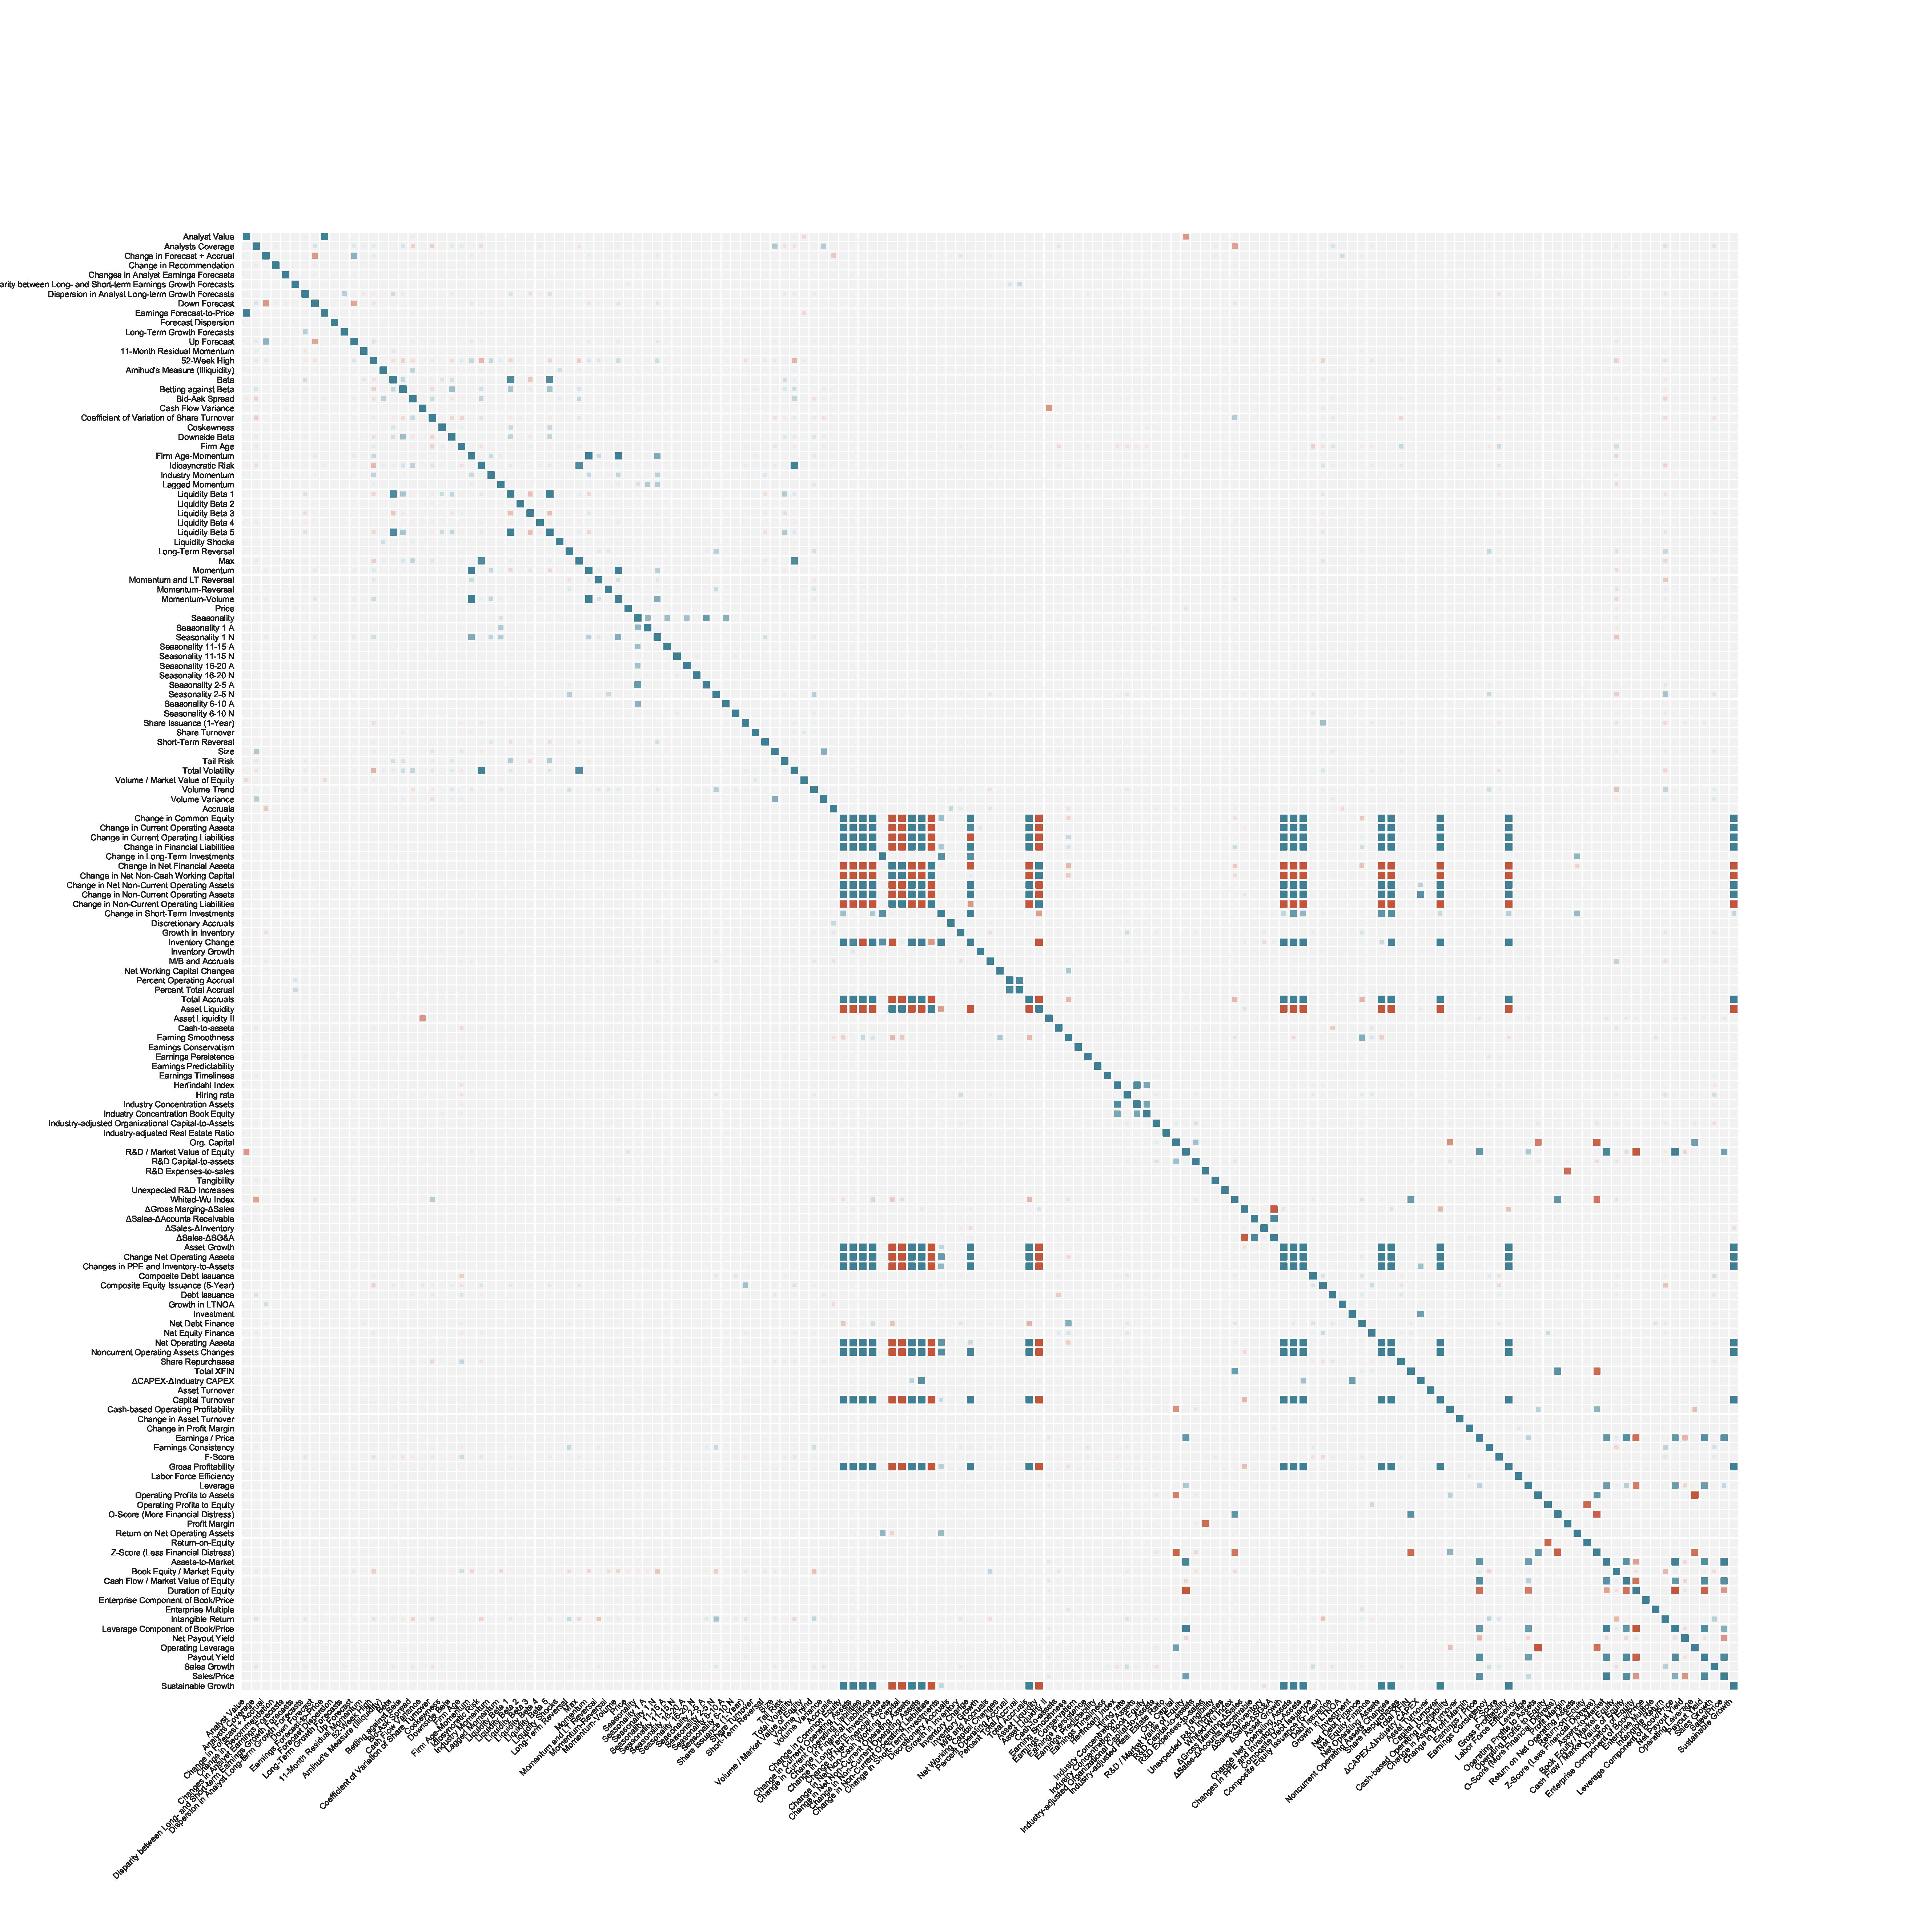
\includegraphics[width=\textwidth,height=\textheight,keepaspectratio]{Figures/corrplot.pdf}
			\caption{Correlation Matrix of the Anomalies}
			\label{fig:corrplot}
		\end{figure}
	\end{center}
	
	
	\begin{center}
		\begin{figure}
			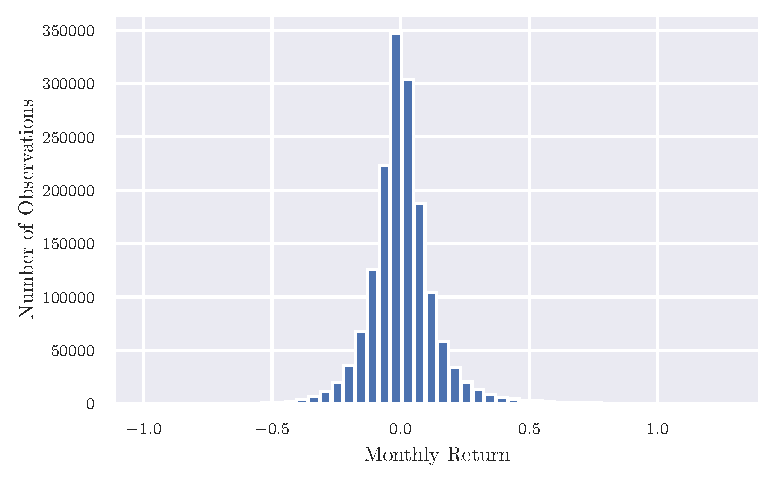
\includegraphics{Figures/hist_returns.pdf}
			\caption{Histogram of Monthly Returns}
			\label{fig:hist_returns}
		\end{figure}
	\end{center}


\section{Methodology}

	I train 5 distinct feed-forward neural networks, each with 9 different random seeds. The architecture and training follows closely \cite{gu2020empirical}, which represents very standard neural networks used in the task of equity return prediction from anomaly data. I compare the performance to that reached in the very same paper. Next, I interpret the neural networks using feature importance and investigate whether this interpretability is robust across different random seeds. I also investigate whether the interpretation of the model is stable in time. This  section describes the methodological issues related, in this order, to the model's architecture, training, performance evaluation and interpretation of the neural networks employed in this thesis.
	
	\subsection{Architecture of the Neural Networks}
	
	The prediction task is to predict stock's return in the following month using a set of the stock's charasteristics calculated as of the current month. My neural networks' architecture is a standard one for this prediction task and identical to \cite{gu2020empirical}. In summary: all networks are feed-forward with the input dimension 30 and the output dimension 1; models of 5 different depths are used, with 1, 2, 3, 4, and 5 hidden layers consisting of 32, 16, 8, 4, and 2 neurons each respectively; all layers are fully connected, with batch-normalization \citep{ioffe2015batch} and ReLU activations on all hidden layers. As this is a regression problem, there is no activation on the output layer. The weights are regularized using l1 penalty. The following explains and motivates these choices in detail, but a reader who is already well-versed in neural network design can easily skip to the next subsection, concerned with training. 
	
	First, let us describe a feed-forward neural network in general terms (e.g., \cite{goodfellow2016deep}). A feed-forward neural network can be represented as directed graph, consisting of several layers. The input layer of $N$ neurons (nodes in the graph). This layer is connected to the next layer of neurons (the first hidden layer) by edges going from each input neuron to each hidden layer neuron. When each neuron of a layer is connected to each neuron in the next layer, we say that the two layers are fully connected. Each edge connecting two neurons is parametrized by a single trainable weight. More hidden layers can be connected to the previous hidden layer in the same fashion. Finally, the last hidden layer is connected, again, fully, to the output layer, which is the final prediction.
	
	This directed graph is a representation of the computation performed by the neural network to get from the input to the output. The values of a given hidden layer, \vec{h}, are computed using the previous layer's values $\vec{x}$, and the matrix of weights on the edges $\vec{W}$ using sum of products: 
	
	\begin{equation}
		\vec{h} = f(\vec{W}\vec{x})
	\end{equation}
	
	or written element-wise, the value of neuron $h_i$ in the hidden layer is computed as 
	
	\begin{equation}
		h_i = f \left( \sum_{j}w_{i,j}x_j \right)
	\end{equation}
	
	where the function $f$ is a non-linear activation function, such as the rectified linear unit (ReLU):
	
	\[
		f(z) = \text{ReLU}(z) =   
			\begin{cases}
				1 & \text{if } z \geq 0\\
				0 & \text{otherwise}
			\end{cases}.
	\]
	
	The output layer is computed using the last hidden layer in the same manner, except in the case of regression there is no activation function. Denoting $\vec{V}$ the weights on the last edges and $\vec{h}$ the output of the last hidden layer, the output of the neural network $\vec{o}$ has the elements: 
	
	\begin{equation}
		o_i = \sum_{j}v_{i,j} h_j.
	\end{equation}
	
	In this thesis, the output is a scalar, so this further simplifies to 
	
	\begin{equation}
		o = \sum_{j}v_{j} h_j.
	\end{equation}
	
	Obviously, in the case of neural network without hidden layers, the model simplifies to linear regression. Adding a hidden layer, which is a non-linear interaction of the previous layer's neurons, the input features are allowed to interact in any manner. Essentially, a hidden layer represents the input features in a sparser manner, generating more abstract, all-encompassing information from them. This information then enters the next hidden layer and the information is made yet more high-level. This continues until the output layer, which produces the most high-level information: the prediction. In this way, the network learns to find relationships between the features such that they predict the target (here, the return) well. The network's depth corresponds to the complexity of the model: the model with a single hidden layer can be considered the least complex one, as the inputs only enter one non-linear interaction, and the complexity increases up to 5 hidden layers, where the most abstract or high-level information is extracted. 
	
	In this thesis, a neural network takes input of 30 real numbers (the stock's characteristics at given time point, dimension of the input layer) and propagates it through the series of hidden layers to produce the return prediction.	A choice must be made as to the number of hidden layers and number of neurons in each layer. While on optimal architecture can be searched for, here it is not necessary, as reaching the best possible performance is not the goal of this thesis. Instead, I follow \cite{gu2020empirical} and use the same numbers of layers and neurons: I train models of 5 different depths (1, 2, 3, 4, and 5 hidden layers), with 32 neurons in the first layer, 16 in the second layer, 8 in the third, 4 in the fourth and 2 in the fifth.  
	
	In addition, I add a batch-normalization layer \citep{ioffe2015batch} after every hidden layer. This changes the above formula for hidden layer values to: 
	
	\begin{equation}
		\vec{h} = \text{ReLU}(\text{BN}(\vec{W}\vec{x}))
	\end{equation}
	
	where $\text{BN}$ represents the batch-normalization operation. The operation simply normalizes its input data (subtracts mean and divides by standard deviation), but the data is split to batches to improve computing speed of the operation. The operation helps with multiple aspects of training the neural networks, as it prevents the values coming out of a hidden layer from being extreme. This helps to regularize the network and also speeds up the training \citep{ioffe2015batch}. 
	
	
	\subsection{Regularization and Training}
	
	Neural networks are non-parametric way of modeling the relationship between the predictors and the predicted variables, in the sense that there is no apriori assumption made about the functional form of the relationship. In fact, the Universal Approximation Theorem shows that with already a single hidden layer, the network outlined above is able to approximate any "well-behaved" function arbitrarily well. This is directly opposed to the linear approach, where we fit the relationship between inputs and outputs assuming a linear functional form. 
	
	This necessarily means that neural networks are prone to overfitting the training data. A number of methods, commonly called regularization, is applied in the architecture and the training process. I use the same regularization techniques as \cite{gu2020empirical}, namely, early stopping, learning rate shrinkage, weight regularization, batch normalization and ensembling.  
	
	To show there is no serious over-fitting, the networks are trained and tuned on a subset of the data (training and validation samples) and evaluated on held-out data (testing sample).
	
	\subsection{Performance Evaluation}
	
	\subsection{Interpretation}
	

	

	
	


